\chapter{System design and implementation}
\label{chapter:system-design}

This chapter presents the entire work of the author. The work is splitted in three parts for the attempt to combine deep neural networks with Q-Learning. The game chosen for experimenting was Tower of Hanoi due to its simplicity and also, the static environment. Then, the values obtained by Q-Learning were used to train a deep convolutional network in combination with the generated frames. Finally, we will try to combine Q-learning algorithm with convolutional networks.



\section{Q-Learning}
\label{sec:ql}
In this section we try to find the optimal policy for playing Tower of Hanoi game. The algorithm start with a pool of actions initialized with {UP, DOWN, LEFT, RIGHT} and a table Q which the values for all (state,action) pairs will be stored. 

The discount factor $\gamma$ is set to 0.95, this future rewards are taking into cosideration when updating the action-value function. The learning rate $\alpha$ is chosen to be 0.1, thus the algorithm can converge to an optimal policy. 

The exploration vs. exploitation problem is solved by using a variable $\epsilon$ which is initialized with 1 (1 is for choosing only random actions and 0 is for choosing the action that can maximize the score). For making the current policy to converge to the optimal policy there was also used a number of iterations setted to 11 and number of episodes per iteration setted to 1000. After each iteration is finished, $\epsilon$ is decreased with 0.1 until it will take the 0-value. This method was used to let the agent explore using random action in the first iteration and after exploit the values learned in the last iterations.

After all the iterations are finished, the algorithm generates a dataset. For each value stored in Q-table, it generates the frame from each coded state.

On the next page, a pseudocode of Q-Learning is presented, which is adapted after the algorithm found in Norvig's book{\cite{norvig}}. The algorithm tries to estimate an optimal action-value function using the $\epsilon$-greedy policy, more exactly, it chooses a random action with probability $\epsilon$ and chooses the optimum action with probability 1-$\epsilon$
\newpage
\begin{algorithm}
	\floatname{algorithm}{Algorithm}
	\caption{Q-Network} \label{alg-code}
	\begin{algorithmic}[1]
		\State set size of Q to with no_states x no_action and initialize it
		\State choose $\epsilon$ between (0,1)
		\State let \textbf{s} be the current state of the game
		\State let \textbf{actions} be a pool with {$a_1$,$a_2$,...,$a_n$}
		\While{game not over}
			\State r = random number between (0,1)
			\If{r < $\epsilon$}
				\State $a_t$ = random action
			\Else
				\State $a_t$ = $argmax_a$ Q(s, a)
			\EndIf
			
			\State $s^\prime$, r = apply_action(a, s)
			\State Q(s,a) = Q(s,a) + $\alpha\cdot$(r + $\gamma\cdot \max_a Q(s^\prime,a^\prime)-Q(s,a)$)
		\EndWhile
	\end{algorithmic}
\end{algorithm}

In the next figures the values resulted from Q are presented. As it can be seen the the optimal policy is it followed. The game allows the picker to move LEFT from first stack and to move RIGHT from last stack (\textbf{e.g.} If the picker points to the first stack and chooses to move LEFT, then the picker will point to the last stack). In fig. \ref{fig:fa} the picker points to the second stack so the optimal action will be to move RIGHT. As we can see the value for RIGHT-action is bigger than the other values. In fig. \ref{fig:fb} the agent has only one move to finish the game, in optimal conditions. Again, if we look at which value is greater than the others we can see that DOWN appears to be 100 which is exactly the value of the reward recieved when an episode is finished. Fig. \ref{fig:fc} represents the initial state of the game, thus as it is expected the game should begin with picking for the first time a disk and that is exactly what Q-Learning is doing.

Another importact aspect which should be mentioned is that the values for actions corresponding to a state \textbf{s} are close. Why? This happens because the game has a static environment and there is no negative reward, thus whatever happens, the agent will always loose or it will be forced to play until the game is finished. The agent can never loose.

\begin{figure}[hp]
\centering
\minipage{0.32\textwidth}
  \frame{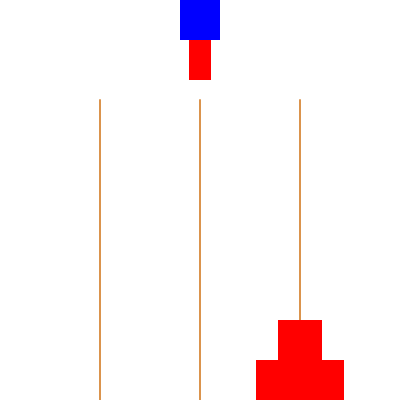
\includegraphics[width=\linewidth]{src/img/results/50}}
  \caption{\newline UP = 90,6534\newline DOWN = 86,8787\newline LEFT = 89,1867\newline RIGHT = 94,2824}\label{fig:fa}
\endminipage\hfill
\minipage{0.32\textwidth}
  \frame{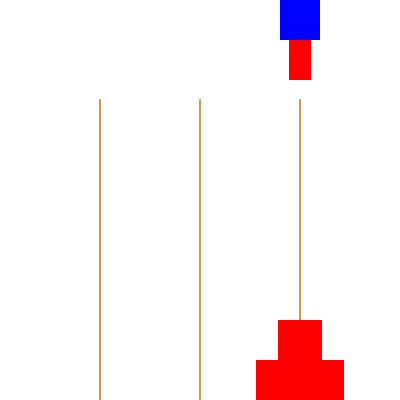
\includegraphics[width=\linewidth]{src/img/results/85}}
  \caption{\newline UP = 97,6530\newline DOWN = 100,0000\newline LEFT = 93,8538\newline RIGHT = 92,5261}\label{fig:fb}
\endminipage\hfill
\minipage{0.32\textwidth}%
  \frame{\includegraphics[width=\linewidth]{src/img/results/155}}
   \caption{\newline UP = 26,3520\newline DOWN = 23,8452\newline LEFT = 23,8897\newline RIGHT = 22,8827}\label{fig:fc}
 
\endminipage
\end{figure}

\newpage
\section{Regression with deep-learning}
This chapter comes with an attempt to discuss various models of architecture that could be suitable for our problem. To see if the network fits the main theme of this paper, one must provide proof that the network model can generalize and is not hitting the ``high variance problem''. In order to come with a scientific proof or at least an empyrical one, several experiments have been made.

\subsection{First attempt}
The model proposed by Yann Lecun et al.\cite{energy-based} was slightly modified in order to map our problem. For the purpose of keeping things clear and well-separated every discussion about a network should be splitted in the next subjects: preprocessing data, chosen model for the network, loss function, training and testing.

For the first attempt, a model used in face detection and pose estimation has been chosen because good results in learning features relevant for object recognition were promised. Also, this model is capable to be applied over large images.

\subsubsection{Data}

In the section \ref{sec:ql}, we generated a dataset of 160 images with 4 labels for each one (Tower of Hanoi has 160 states and offers 4 possible actions). In this section we try to build a convolutional neural network capable of predicting those values from images. This is made for the sake of bringing a strong argumentation that our network model is capable of learning features from the dataset and it is not conducting to a ``dead'' network which is ``overlearning'' and can not be used on new samples.

First step was to resolve the problem of the small number of samples (160) from dataset. This has been solved by generating 64 another datasets (to achive approximately 10,000 samples) from the original one with noise added or color changed. In this way we can ensure that the network is capable of learning features dependent of size in this case.

The next figure(\ref{fig:155}) represent a state of the game and the next ones(\ref{fig:states}) represent alterated images with noise added and color changed.

\begin{figure}[h]
	\begin{center}
		\frame{\includegraphics[width=130px,height=130px]{src/img/system-design/155}}
		\caption{Initial state of the game ``Tower of Hanoi''} \label{fig:155}
    \end{center}
\end{figure}

\begin{figure}[h]
	\begin{center}
		\frame{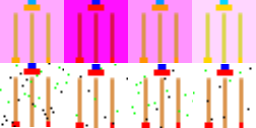
\includegraphics[width=253px,height=126px]{src/img/system-design/states}}
		\caption{Alterated dataset} \label{fig:states}
    \end{center}
\end{figure}
\newpage

For the preprocessing data various problems have been attemped. First of all, there is a large discussion on the RGB vs. YUV topic. This paper implements the YUV transformation based on the assumption that luminance should be separated from chrominance. If features dependent of color should be learned, then the neurons connected with the chrominance pixels will be activated, otherwise the neurons connected with luminance pixels will be activated. Both type of channels are kept in the attempt to make an algorithm that could generalize very well. Also, the YUV color is more closer to the human vision than RGB. 

The decision to not work with 1-channels colors space like grayscale are well-founded. There are games that size should not be a feature which should be learned and in this cases we are interested in learning features dependent of color.

The next step was to normalize the images for aligning the range of pixel intensity values to a normal distribution. With other words, the histogram of the images are stretched and the contrast is improved in order to get sharp edges.

The normalization of the images implies computing the mean and the standard deviation. These values are computed for the training dataset for each channel. Then, we add the mean and divide it with standard deviation. This operation is applied on each channel on both datasets (train and test).

Another way to improve the contrast is ussing a gaussian matrix which follows a gaussian distribution, as it is clear from its name. The gaussian distribution state that average things should occur frequently and extreme things should occur rare. The gaussian matrix will slide all over the image and will modify the pixel values such that the pixels from the middle of the neighbourhood will be more important than the pixel values from the edge of the gaussian matrix. If the edge pixel values have a zero importance than the result image will be exactly as the initial image.

On the another hand, labels were also needed to be processed. Because of the formula for estimating the action-value function (Q) different ranges of values were generated. For example, if we have to do regression on values as 0,..., 100 there would not be a problem because the delta range is $10^2$, but the values generated were following a delta range of $10^5$. This can cause instability to the network. These being said, the paper proposes to bring the values to the same range using logarithm function and of course, to normalize them to follow the normal distribution.

Data was also shuffled to avoid having consecutive states from the game

\begin{figure}[h]
	\begin{center}
		\includegraphics[width=480px,height=103px]{src/img/system-design/myarch}
		\caption{ConvNet Architecture} \label{fig:myarch}
    \end{center}
\end{figure}